\documentclass[10pt,fleqn]{article} % Default font size and left-justified equations
\usepackage[%
    pdftitle={Informatique : Tris d'une liste de valeurs numériques},
    pdfauthor={Xavier Pessoles}]{hyperref}


%%%%%%%%%%%%%%%%%%%%%%%%%%%%%%%%%%%%%%%%%
% Original author:
% Mathias Legrand (legrand.mathias@gmail.com) with modifications by:
% Vel (vel@latextemplates.com)
% License:
% CC BY-NC-SA 3.0 (http://creativecommons.org\newtheorem{rappelT}{Rappel}[section]/licenses/by-nc-sa/3.0/)
%%%%%%%%%%%%%%%%%%%%%%%%%%%%%%%%%%%%%%%%%

%----------------------------------------------------------------------------------------
%	VARIOUS REQUIRED PACKAGES AND CONFIGURATIONS
%----------------------------------------------------------------------------------------

\usepackage[top=2.5cm,bottom=2cm,left=2cm,right=2cm,headsep=40pt,a4paper]{geometry} % Page margins

\usepackage{graphicx} % Required for including pictures
\graphicspath{{images/}} % Specifies the directory where pictures are stored
\usepackage{float}

\usepackage{lipsum} % Inserts dummy text

\usepackage{tikz} % Required for drawing custom shapes

\usepackage[french]{babel} % English language/hyphenation
\frenchbsetup{StandardLists=true} % Pour éviter la collision babel enumitem pour les listes

\usepackage{enumitem} % Customize lists
\setlist{nolistsep} % Reduce spacing between bullet points and numbered lists

\usepackage{booktabs} % Required for nicer horizontal rules in tables

\usepackage{colortbl} % Couleur dans les tableaux

\usepackage{xcolor} % Required for specifying colors by name
%\definecolor{ocre}{RGB}{243,102,25} % Define the orange color used for highlighting throughout the book
\definecolor{ocre}{RGB}{49,133,156} % Couleur ''bleue''
\definecolor{violetf}{RGB}{112,48,160} % Couleur ''violet''
\usepackage{enumitem}
\usepackage{pifont} % Pour les dinglist
\usepackage{multicol}
\usepackage{array} % Centrage vertical dans les tableaux

%----------------------------------------------------------------------------------------
%	FONTS
%----------------------------------------------------------------------------------------

\usepackage{avant} % Use the Avantgarde font for headings
%\usepackage{times} % Use the Times font for headings
%\usepackage{mathptmx} % Use the Adobe Times Roman as the default text font together with math symbols from the Sym­bol, Chancery and Com­puter Modern fonts
\usepackage[adobe-utopia]{mathdesign}
\usepackage{microtype} % Slightly tweak font spacing for aesthetics
\usepackage[utf8]{inputenc} % Required for including letters with accents
\usepackage[T1]{fontenc} % Use 8-bit encoding that has 256 glyphs

%----------------------------------------------------------------------------------------
%	BIBLIOGRAPHY AND INDEX
%----------------------------------------------------------------------------------------

\usepackage[style=alphabetic,citestyle=numeric,sorting=nyt,sortcites=true,autopunct=true,babel=hyphen,hyperref=true,abbreviate=false,backref=true,backend=biber]{biblatex}
\addbibresource{bibliography.bib} % BibTeX bibliography file
\defbibheading{bibempty}{}

\usepackage{calc} % For simpler calculation - used for spacing the index letter headings correctly
\usepackage{makeidx} % Required to make an index
\makeindex % Tells LaTeX to create the files required for indexing

%----------------------------------------------------------------------------------------
%	MAIN TABLE OF CONTENTS
%----------------------------------------------------------------------------------------

\usepackage{titletoc} % Required for manipulating the table of contents

\setcounter{tocdepth}{2}     % Dans la table des matieres
\setcounter{secnumdepth}{2}

\contentsmargin{0cm} % Removes the default margin

% Part text styling
\titlecontents{part}[0cm]
{\addvspace{20pt}\centering\large\bfseries}
{}
{}
{}

% Chapter text styling
\titlecontents{chapter}[1.25cm] % Indentation
{\addvspace{12pt}\large\sffamily\bfseries} % Spacing and font options for chapters
{\color{ocre!60}\contentslabel[\Large\thecontentslabel]{1.25cm}\color{ocre}} % Chapter number
{\color{ocre}}  
{\color{ocre!60}\normalsize\;\titlerule*[.5pc]{.}\;\thecontentspage} % Page number

% Section text styling
\titlecontents{section}[1.25cm] % Indentation
{\addvspace{3pt}\sffamily\bfseries} % Spacing and font options for sections
{\color{ocre!60}\contentslabel[\thecontentslabel]{1.25cm} \color{ocre}} % Section number
{\color{ocre}}
{\hfill\color{ocre!60}\thecontentspage} % Page number
[]

% Subsection text styling
\titlecontents{subsection}[1.25cm] % Indentation
{\addvspace{1pt}\sffamily\small} % Spacing and font options for subsections
{\contentslabel[\thecontentslabel]{1.25cm}} % Subsection number
{}
{\ \titlerule*[.5pc]{.}\;\thecontentspage} % Page number
[]


% Subsection text styling
\titlecontents{subsubsection}[1.25cm] % Indentation
{\addvspace{1pt}\sffamily\small} % Spacing and font options for subsections
{\contentslabel[\thecontentslabel]{1.25cm}} % Subsection number
{}
{\ \titlerule*[.5pc]{.}\;\thecontentspage} % Page number
[]

% List of figures
\titlecontents{figure}[0em]
{\addvspace{-5pt}\sffamily}
{\thecontentslabel\hspace*{1em}}
{}
{\ \titlerule*[.5pc]{.}\;\thecontentspage}
[]

% List of tables
\titlecontents{table}[0em]
{\addvspace{-5pt}\sffamily}
{\thecontentslabel\hspace*{1em}}
{}
{\ \titlerule*[.5pc]{.}\;\thecontentspage}
[]

%----------------------------------------------------------------------------------------
%	MINI TABLE OF CONTENTS IN PART HEADS
%----------------------------------------------------------------------------------------

% Chapter text styling
\titlecontents{lchapter}[0em] % Indenting
{\addvspace{15pt}\large\sffamily\bfseries} % Spacing and font options for chapters
{\color{ocre}\contentslabel[\Large\thecontentslabel]{1.25cm}\color{ocre}} % Chapter number
{}  
{\color{ocre}\normalsize\sffamily\bfseries\;\titlerule*[.5pc]{.}\;\thecontentspage} % Page number

% Section text styling
\titlecontents{lsection}[0em] % Indenting
{\sffamily\small} % Spacing and font options for sections
{\contentslabel[\thecontentslabel]{1.25cm}} % Section number
{}
{}

% Subsection text styling
\titlecontents{lsubsection}[.5em] % Indentation
{\normalfont\footnotesize\sffamily} % Font settings
{}
{}
{}

%----------------------------------------------------------------------------------------
%	PAGE HEADERS
%----------------------------------------------------------------------------------------

\usepackage{fancyhdr} % Required for header and footer configuration



\pagestyle{fancy}
 \renewcommand{\headrulewidth}{0pt}
 \fancyhead{}
 \fancyhead[L]{%
 \noindent\begin{minipage}[c]{2.6cm}%
 
\includegraphics[width=2cm]{png/logo_lycee.png}%
 \end{minipage}}

\fancyhead[C]{\rule{8cm}{.5pt}}

 \fancyhead[R]{%
 \noindent\begin{minipage}[c]{3cm}
 \begin{flushright}
 \footnotesize{\textit{\textsf{\xxtete}}}%
 \end{flushright}
 \end{minipage}
}


\fancyfoot[C]{\rule{12cm}{.5pt}}
\renewcommand{\footrulewidth}{0.2pt}
\fancyfoot[C]{\footnotesize{\bfseries \thepage}}
\fancyfoot[L]{ 
\begin{minipage}[c]{.2\linewidth}
\noindent\footnotesize{{\xxauteur}}
\end{minipage}}


\fancyfoot[R]{\footnotesize{\xxpied}
\ifthenelse{\isodd{\value{page}}}{
\begin{tikzpicture}[overlay]
\node[shape=rectangle, 
      rounded corners = .25 cm,
	  draw= ocre,
	  line width=2pt, 
	  fill = ocre!10,
	  minimum width  = 2.5cm,
	  minimum height = 3cm,] at (\xxposongletx,\xxposonglety) {};
\node at (\xxposonglettext,\xxposonglety) {\rotatebox{90}{\textbf{\large\color{ocre}{\xxonglet}}}};
%{};
\end{tikzpicture}}{}
}
%
%
%
% Removes the header from odd empty pages at the end of chapters
\makeatletter
\renewcommand{\cleardoublepage}{
\clearpage\ifodd\c@page\else
\hbox{}
\vspace*{\fill}
\thispagestyle{empty}
\newpage
\fi}

\fancypagestyle{plain}{%
\fancyhf{} % vide l’en-tête et le pied~de~page.
%\fancyfoot[C]{\bfseries \thepage} % numéro de la page en cours en gras
% et centré en pied~de~page.
\fancyfoot[R]{\footnotesize{\xxpied}}
\fancyfoot[C]{\rule{12cm}{.5pt}}
\renewcommand{\footrulewidth}{0.2pt}
\fancyfoot[C]{\footnotesize{\bfseries \thepage}}
\fancyfoot[L]{ 
\begin{minipage}[c]{.2\linewidth}
\noindent\footnotesize{{\xxauteur}}
\end{minipage}}}



%----------------------------------------------------------------------------------------
%	THEOREM STYLES
%----------------------------------------------------------------------------------------

% Conflit avec la police adobe
%\usepackage{amsmath,amsfonts,amssymb,amsthm} % For math equations, theorems, symbols, etc
\usepackage{amsmath,amsthm}

\newcommand{\intoo}[2]{\mathopen{]}#1\,;#2\mathclose{[}}
\newcommand{\ud}{\mathop{\mathrm{{}d}}\mathopen{}}
\newcommand{\intff}[2]{\mathopen{[}#1\,;#2\mathclose{]}}
%\newtheorem{notation}{Notation}[chapter]
\newtheorem{notation}{Notation}[section]

% Boxed/framed environments
\newtheoremstyle{ocrenumbox}% % Theorem style name
{0pt}% Space above
{0pt}% Space below
{\normalfont}% % Body font
{}% Indent amount
{\small\bf\sffamily\color{ocre}}% % Theorem head font
{\;}% Punctuation after theorem head
{0.25em}% Space after theorem head
{\small\sffamily\color{ocre}\thmname{#1}\nobreakspace\thmnumber%{\@ifnotempty{#1}{}\@upn{#2}}% Theorem text (e.g. Theorem 2.1)
\thmnote{\nobreakspace\the\thm@notefont\sffamily\bfseries\color{black}---\nobreakspace#3.}} % Optional theorem note
\renewcommand{\qedsymbol}{$\blacksquare$}% Optional qed square


% Boite pour les corriges
\newtheoremstyle{correctionbox}% % Theorem style name
{0pt}% Space above
{0pt}% Space below
{\normalfont}% % Body font
{}% Indent amount
{\small\bf\sffamily\color{violet}}% % Theorem head font
{\;}% Punctuation after theorem head
{0.25em}% Space after theorem head
{\small\sffamily\color{ocre}\thmname{#1}\nobreakspace\thmnumber%{\@ifnotempty{#1}{}\@upn{#2}}% Theorem text (e.g. Theorem 2.1)
\thmnote{\nobreakspace\the\thm@notefont\sffamily\bfseries\color{black}---\nobreakspace#3.}} % Optional theorem note
\renewcommand{\qedsymbol}{$\blacksquare$}% Optional qed square



\newtheoremstyle{blacknumex}% Theorem style name
{5pt}% Space above
{5pt}% Space below
{\normalfont}% Body font
{} % Indent amount
{\small\bf\sffamily}% Theorem head font
{\;}% Punctuation after theorem head
{0.25em}% Space after theorem head
{\small\sffamily{\tiny\ensuremath{\blacksquare}}\nobreakspace\thmname{#1}\nobreakspace\thmnumber%{\@ifnotempty{#1}{}\@upn{#2}}% Theorem text (e.g. Theorem 2.1)
\thmnote{\nobreakspace\the\thm@notefont\sffamily\bfseries---\nobreakspace#3.}}% Optional theorem note

\newtheoremstyle{blacknumbox} % Theorem style name
{0pt}% Space above
{0pt}% Space below
{\normalfont}% Body font
{}% Indent amount
{\small\bf\sffamily}% Theorem head font
{\;}% Punctuation after theorem head
{0.25em}% Space after theorem head
{\small\sffamily\thmname{#1}\nobreakspace 
\thmnote{\nobreakspace\the\thm@notefont\sffamily\bfseries---\nobreakspace#3.}}% Optional theorem note

% Non-boxed/non-framed environments
\newtheoremstyle{ocrenum}% % Theorem style name
{5pt}% Space above
{5pt}% Space below
{\normalfont}% % Body font
{}% Indent amount
{\small\bf\sffamily\color{ocre}}% % Theorem head font
{\;}% Punctuation after theorem head
{0.25em}% Space after theorem head
{\small\sffamily\color{ocre}\thmname{#1}\nobreakspace%\thmnumber{\@ifnotempty{#1}{}\@upn{#2}}% Theorem text (e.g. Theorem 2.1)
\thmnote{\nobreakspace\the\thm@notefont\sffamily\bfseries\color{black}---\nobreakspace#3.}} % Optional theorem note
\renewcommand{\qedsymbol}{$\blacksquare$}% Optional qed square
\makeatother

% Environnement pour les titres de parties
\newtheoremstyle{partiebox} 
{0pt}% Space above
{0pt}% Space below
{\normalfont}% Body font
{}% Indent amount
{\small\bf\sffamily}% Theorem head font
{\;}% Punctuation after theorem head
{0.25em}% Space after theorem head




% Defines the theorem text style for each type of theorem to one of the three styles above
\newcounter{dummy} 
\numberwithin{dummy}{section}
\theoremstyle{ocrenumbox}
%\newtheorem{theoremeT}[dummy]{Théorème}
\newtheorem{theoremeT}[dummy]{Théorème}
\newtheorem{resultatT}[dummy]{Résultat}
\newtheorem{savoirT}[dummy]{Savoir}
\newtheorem{methodeT}[dummy]{Méthode}
\newtheorem{objectifT}[dummy]{Objectif}
%\newtheorem{problem}{Problem}[chapter]
\newtheorem{problem}{Problem}[section]
%\newtheorem{exerciseT}{Exercise}[chapter]
\newtheorem{exerciseT}{Exercice}[section]

\theoremstyle{blacknumex}
%\newtheorem{exampleT}{Example}[chapter]
\newtheorem{exempleT}{Exemple}[section]
\newtheorem{termT}{Terminal\\}[section]
\newtheorem{pyT}{Python\\}[section]
\newtheorem{sciT}{Scilab\\}[section]
\newtheorem{pseudoT}{Pseudo Code\\}[section]
\newtheorem{sqlT}{SQL\\}[section]

\theoremstyle{blacknumbox}
%\newtheorem{vocabulary}{Vocabulary}[chapter]
\newtheorem{vocabulary}{Vocabulaire}[section]
%\newtheorem{definitionT}{Definition}[section]
\newtheorem{definitionT}{Définition}[section]
\newtheorem{rappelT}{Rappel}[section]
\newtheorem{demoT}{Démonstration}[section]
\newtheorem{corollaryT}[dummy]{Corollaire}
\newtheorem{hypoT}{Hypothèse(s)}

\theoremstyle{ocrenum}
\newtheorem{proposition}[dummy]{Proposition}

\theoremstyle{partiebox}
\newtheorem{titrepartieT}[]{}
\newtheorem{titrechapitreT}[]{}

\theoremstyle{correctionbox}
\newtheorem{correctionT}[dummy]{\color{violet}{Correction}}

%----------------------------------------------------------------------------------------
%	DEFINITION OF COLORED BOXES
%----------------------------------------------------------------------------------------

\RequirePackage[framemethod=tikz]{mdframed} % Required for creating the theorem, definition, exercise and corollary boxes

% Theorem box
\newmdenv[skipabove=7pt,
skipbelow=7pt,
backgroundcolor=ocre!10,
linecolor=ocre,
innerleftmargin=5pt,
innerrightmargin=5pt,
innertopmargin=5pt,
leftmargin=0cm,
rightmargin=0cm,
innerbottommargin=5pt]{tBox}


% Correction
\newmdenv[skipabove=7pt,
skipbelow=7pt,
backgroundcolor=violet!10,
linecolor=violet,
innerleftmargin=5pt,
innerrightmargin=5pt,
innertopmargin=5pt,
leftmargin=0cm,
rightmargin=0cm,
innerbottommargin=5pt]{coBox}


% Exercise box	  
\newmdenv[skipabove=7pt,
skipbelow=7pt,
rightline=false,
leftline=true,
topline=false,
bottomline=false,
backgroundcolor=ocre!10,
linecolor=ocre,
innerleftmargin=5pt,
innerrightmargin=5pt,
innertopmargin=5pt,
innerbottommargin=5pt,
leftmargin=0cm,
rightmargin=0cm,
linewidth=4pt]{eBox}	

% Definition box
\newmdenv[skipabove=7pt,
skipbelow=7pt,
rightline=false,
leftline=true,
topline=false,
bottomline=false,
backgroundcolor=ocre!10,
linecolor=ocre,
innerleftmargin=5pt,
innerrightmargin=5pt,
innertopmargin=1pt,
leftmargin=0cm,
rightmargin=0cm,
linewidth=4pt,
innerbottommargin=0pt]{dBox}	

% Demonstration box
\newmdenv[skipabove=7pt,
skipbelow=7pt,
rightline=false,
leftline=true,
topline=false,
bottomline=false,
%backgroundcolor=ocre!10,
linecolor=ocre,
innerleftmargin=5pt,
innerrightmargin=5pt,
innertopmargin=0pt,
leftmargin=0cm,
rightmargin=0cm,
linewidth=4pt,
innerbottommargin=0pt]{demoBox}	

% Corollary box
\newmdenv[skipabove=7pt,
skipbelow=7pt,
rightline=false,
leftline=true,
topline=false,
bottomline=false,
linecolor=gray,
backgroundcolor=black!5,
innerleftmargin=5pt,
innerrightmargin=5pt,
innertopmargin=5pt,
leftmargin=0cm,
rightmargin=0cm,
linewidth=4pt,
innerbottommargin=5pt]{cBox}


% Hypothèses
\newmdenv[skipabove=7pt,
skipbelow=7pt,
rightline=false,
leftline=true,
topline=false,
bottomline=false,
linecolor=gray,
backgroundcolor=black!5,
innerleftmargin=5pt,
innerrightmargin=5pt,
innertopmargin=5pt,
leftmargin=0cm,
rightmargin=0cm,
linewidth=4pt,
innerbottommargin=5pt]{hyBox}


% Boite pour le titre de la partie (pBox)
\newmdenv[skipabove=7pt,
skipbelow=7pt,
rightline=true,
leftline=false,
topline=false,
bottomline=false,
linecolor=ocre,
backgroundcolor=none,
innerleftmargin=5pt,
innerrightmargin=5pt,
innertopmargin=5pt,
leftmargin=0cm,
rightmargin=0cm,
linewidth=4pt,
innerbottommargin=5pt]{pBox}

% Boite pour le titre du chapitre (chBox)
\newmdenv[skipabove=7pt,
skipbelow=7pt,
rightline=false,
leftline=true,
topline=false,
bottomline=false,
linecolor=ocre,
%backgroundcolor=black!5,
innerleftmargin=5pt,
innerrightmargin=5pt,
innertopmargin=5pt,
leftmargin=0cm,
rightmargin=0cm,
linewidth=4pt,
innerbottommargin=5pt]{chBox}


% Boite pour les exemples
\newmdenv[skipabove=7pt,
skipbelow=7pt,
rightline=false,
leftline=true,
topline=false,
bottomline=false,
linecolor=gray,
backgroundcolor=white,
innerleftmargin=5pt,
innerrightmargin=5pt,
innertopmargin=5pt,
leftmargin=0cm,
rightmargin=0cm,
linewidth=4pt,
innerbottommargin=5pt]{exBox}

% Boite pour le terminal
\newmdenv[skipabove=7pt,
skipbelow=7pt,
rightline=false,
leftline=true,
topline=false,
bottomline=false,
linecolor=gray,
backgroundcolor=white,
innerleftmargin=5pt,
innerrightmargin=5pt,
innertopmargin=5pt,
leftmargin=0cm,
rightmargin=0cm,
linewidth=4pt,
innerbottommargin=5pt]{termBox}


% Boite pour Python
\newmdenv[skipabove=7pt,
skipbelow=7pt,
rightline=false,
leftline=true,
topline=false,
bottomline=false,
linecolor=gray,
backgroundcolor=white,
innerleftmargin=5pt,
innerrightmargin=5pt,
innertopmargin=5pt,
leftmargin=0cm,
rightmargin=0cm,
linewidth=4pt,
innerbottommargin=5pt]{pyBox}

% Boite pour scilab
\newmdenv[skipabove=7pt,
skipbelow=7pt,
rightline=false,
leftline=true,
topline=false,
bottomline=false,
linecolor=gray,
backgroundcolor=white,
innerleftmargin=5pt,
innerrightmargin=5pt,
innertopmargin=5pt,
leftmargin=0cm,
rightmargin=0cm,
linewidth=4pt,
innerbottommargin=5pt]{sciBox}


% Boite pour pseudo
\newmdenv[skipabove=7pt,
skipbelow=7pt,
rightline=false,
leftline=true,
topline=false,
bottomline=false,
linecolor=gray,
backgroundcolor=white,
innerleftmargin=5pt,
innerrightmargin=5pt,
innertopmargin=5pt,
leftmargin=0cm,
rightmargin=0cm,
linewidth=4pt,
innerbottommargin=5pt]{pseudoBox}

% Boite pour pseudo
\newmdenv[skipabove=7pt,
skipbelow=7pt,
rightline=false,
leftline=true,
topline=false,
bottomline=false,
linecolor=gray,
backgroundcolor=white,
innerleftmargin=5pt,
innerrightmargin=5pt,
innertopmargin=5pt,
leftmargin=0cm,
rightmargin=0cm,
linewidth=4pt,
innerbottommargin=5pt]{sqlBox}


% Creates an environment for each type of theorem and assigns it a theorem text style from the "Theorem Styles" section above and a colored box from above
\newenvironment{theorem}{\begin{tBox}\begin{theoremeT}}{\end{theoremeT}\end{tBox}}
\newenvironment{resultat}{\begin{tBox}\begin{resultatT}}{\end{resultatT}\end{tBox}}
\newenvironment{methode}{\begin{tBox}\begin{methodeT}}{\end{methodeT}\end{tBox}}
\newenvironment{savoir}{\begin{tBox}\begin{savoirT}}{\end{savoirT}\end{tBox}}
\newenvironment{obj}{\begin{tBox}\begin{objectifT}}{\end{objectifT}\end{tBox}}
\newenvironment{corrige}{\begin{coBox}\begin{correctionT}}{\end{correctionT}\end{coBox}}
\newenvironment{exercise}{\begin{eBox}\begin{exerciseT}}{\hfill{\color{ocre}\tiny\ensuremath{\blacksquare}}\end{exerciseT}\end{eBox}}				  
\newenvironment{exercice}{\begin{eBox}\begin{exerciseT}}{\hfill{\color{ocre}\tiny\ensuremath{\blacksquare}}\end{exerciseT}\end{eBox}}				  

\newenvironment{definition}{\begin{dBox}\begin{definitionT}}{\end{definitionT}\end{dBox}}	
\newenvironment{defi}{\begin{dBox}\begin{definitionT}}{\end{definitionT}\end{dBox}}	
\newenvironment{demo}{\begin{demoBox}\begin{demoT}}{\end{demoT}\end{demoBox}}	
\newenvironment{rappel}{\begin{dBox}\begin{rappelT}}{\end{rappelT}\end{dBox}}	
%\newenvironment{exemple}{\begin{exempleT}}{\hfill{\tiny\ensuremath{\blacksquare}}\end{exempleT}}		
\newenvironment{corollary}{\begin{cBox}\begin{corollaryT}}{\end{corollaryT}\end{cBox}}
\newenvironment{hypo}{\begin{hyBox}\begin{hypoT}}{\end{hypoT}\end{hyBox}}	\newenvironment{exemple}{\begin{exBox}\begin{exempleT}}{\hfill{\tiny\ensuremath{\blacksquare}}\end{exempleT}\end{exBox}}	
\newenvironment{titrepartie}{\begin{pBox}\begin{titrepartieT}}{\end{titrepartieT}\end{pBox}}	
\newenvironment{titrechapitre}{\begin{chBox}\begin{titrechapitreT}}{\end{titrechapitreT}\end{chBox}}	

\newenvironment{term}{ \begin{termBox}\begin{termT}}{\end{termT}\end{termBox}}
\newenvironment{py}{ \begin{pyBox}\begin{pyT}}{\end{pyT}\end{pyBox}}
\newenvironment{sci}{ \begin{sciBox}\begin{sciT}}{\end{sciT}\end{sciBox}}
\newenvironment{pseudo}{ \begin{pseudoBox}\begin{pseudoT}}{\end{pseudoT}\end{pseudoBox}}
\newenvironment{envsql}{ \begin{sqlBox}\begin{sqlT}}{\end{sqlT}\end{sqlBox}}


%----------------------------------------------------------------------------------------
%	REMARK ENVIRONMENT
%----------------------------------------------------------------------------------------

\newenvironment{remark}{\par\vspace{10pt}\small % Vertical white space above the remark and smaller font size
\begin{list}{}{
\leftmargin=35pt % Indentation on the left
\rightmargin=25pt}\item\ignorespaces % Indentation on the right
\makebox[-2.5pt]{\begin{tikzpicture}[overlay]
\node[draw=ocre!60,line width=1pt,circle,fill=ocre!25,font=\sffamily\bfseries,inner sep=2pt,outer sep=0pt] at (-15pt,0pt){\textcolor{ocre}{R}};\end{tikzpicture}} % Orange R in a circle
\advance\baselineskip -1pt}{\end{list}\vskip5pt} % Tighter line spacing and white space after remark

\newenvironment{rem}{\par\vspace{10pt}\small % Vertical white space above the remark and smaller font size
\begin{list}{}{
\leftmargin=35pt % Indentation on the left
\rightmargin=25pt}\item\ignorespaces % Indentation on the right
\makebox[-2.5pt]{\begin{tikzpicture}[overlay]
\node[draw=ocre!60,line width=1pt,circle,fill=ocre!25,font=\sffamily\bfseries,inner sep=2pt,outer sep=0pt] at (-15pt,0pt){\textcolor{ocre}{R}};\end{tikzpicture}} % Orange R in a circle
\advance\baselineskip -1pt}{\end{list}\vskip5pt} % Tighter line spacing and white space after remark


\newenvironment{warn}{\par\vspace{10pt}\small % Vertical white space above the remark and smaller font size
\begin{list}{}{
\leftmargin=35pt % Indentation on the left
\rightmargin=25pt}\item\ignorespaces % Indentation on the right
\makebox[-2.5pt]{\begin{tikzpicture}[overlay]
\node[draw=red!60,line width=1pt,circle,fill=red!25,font=\sffamily\bfseries,inner sep=2pt,outer sep=0pt] at (-15pt,0pt){\textcolor{black}{!}};\end{tikzpicture}} % Point d'exclamation dans un cercle
\advance\baselineskip -1pt}{\end{list}\vskip5pt} % Tighter line spacing and white space after remark


%----------------------------------------------------------------------------------------
%	SECTION NUMBERING IN THE MARGIN
%----------------------------------------------------------------------------------------
\setcounter{secnumdepth}{3}
\setcounter{tocdepth}{2}



\makeatletter
\renewcommand{\@seccntformat}[1]{\llap{\textcolor{ocre}{\csname the#1\endcsname}\hspace{1em}}}                    
\renewcommand{\section}{\@startsection{section}{1}{\z@}
{-4ex \@plus -1ex \@minus -.4ex}
{1ex \@plus.2ex }
{\normalfont\large\sffamily\bfseries}}
\renewcommand{\subsection}{\@startsection {subsection}{2}{\z@}
{-3ex \@plus -0.1ex \@minus -.4ex}
{0.5ex \@plus.2ex }
{\normalfont\sffamily\bfseries}}
\renewcommand{\subsubsection}{\@startsection {subsubsection}{3}{\z@}
{-2ex \@plus -0.1ex \@minus -.2ex}
{.2ex \@plus.2ex }
{\normalfont\small\sffamily\bfseries}}                        
\renewcommand\paragraph{\@startsection{paragraph}{4}{\z@}
{-2ex \@plus-.2ex \@minus .2ex}
{.1ex}
{\normalfont\small\sffamily\bfseries}}

%----------------------------------------------------------------------------------------
%	PART HEADINGS
%----------------------------------------------------------------------------------------


%----------------------------------------------------------------------------------------
%	CHAPTER HEADINGS
%----------------------------------------------------------------------------------------

% \newcommand{\thechapterimage}{}%
% \newcommand{\chapterimage}[1]{\renewcommand{\thechapterimage}{#1}}%
% \def\@makechapterhead#1{%
% {\parindent \z@ \raggedright \normalfont
% \ifnum \c@secnumdepth >\m@ne
% \if@mainmatter
% \begin{tikzpicture}[remember picture,overlay]
% \node at (current page.north west)
% {\begin{tikzpicture}[remember picture,overlay]
% \node[anchor=north west,inner sep=0pt] at (0,0) {\includegraphics[width=\paperwidth]{\thechapterimage}};
% \draw[anchor=west] (\Gm@lmargin,-9cm) node [line width=2pt,rounded corners=15pt,draw=ocre,fill=white,fill opacity=0.5,inner sep=15pt]{\strut\makebox[22cm]{}};
% \draw[anchor=west] (\Gm@lmargin+.3cm,-9cm) node {\huge\sffamily\bfseries\color{black}\thechapter. #1\strut};
% \end{tikzpicture}};
% \end{tikzpicture}
% \else
% \begin{tikzpicture}[remember picture,overlay]
% \node at (current page.north west)
% {\begin{tikzpicture}[remember picture,overlay]
% \node[anchor=north west,inner sep=0pt] at (0,0) {\includegraphics[width=\paperwidth]{\thechapterimage}};
% \draw[anchor=west] (\Gm@lmargin,-9cm) node [line width=2pt,rounded corners=15pt,draw=ocre,fill=white,fill opacity=0.5,inner sep=15pt]{\strut\makebox[22cm]{}};
% \draw[anchor=west] (\Gm@lmargin+.3cm,-9cm) node {\huge\sffamily\bfseries\color{black}#1\strut};
% \end{tikzpicture}};
% \end{tikzpicture}
% \fi\fi\par\vspace*{270\p@}}}

%-------------------------------------------

\def\@makeschapterhead#1{%
\begin{tikzpicture}[remember picture,overlay]
\node at (current page.north west)
{\begin{tikzpicture}[remember picture,overlay]
\node[anchor=north west,inner sep=0pt] at (0,0) {\includegraphics[width=\paperwidth]{\thechapterimage}};
\draw[anchor=west] (\Gm@lmargin,-9cm) node [line width=2pt,rounded corners=15pt,draw=ocre,fill=white,fill opacity=0.5,inner sep=15pt]{\strut\makebox[22cm]{}};
\draw[anchor=west] (\Gm@lmargin+.3cm,-9cm) node {\huge\sffamily\bfseries\color{black}#1\strut};
\end{tikzpicture}};
\end{tikzpicture}
\par\vspace*{270\p@}}
\makeatother

%----------------------------------------------------------------------------------------
%	HYPERLINKS IN THE DOCUMENTS
%----------------------------------------------------------------------------------------


\hypersetup{hidelinks,backref=true,pagebackref=true,hyperindex=true,colorlinks=false,breaklinks=true,urlcolor= ocre,bookmarks=true,bookmarksopen=false,pdftitle={Title},pdfauthor={Author}}
\usepackage{bookmark}
\bookmarksetup{
open,
numbered,
addtohook={%
\ifnum\bookmarkget{level}=0 % chapter
\bookmarksetup{bold}%
\fi
\ifnum\bookmarkget{level}=-1 % part
\bookmarksetup{color=ocre,bold}%
\fi
}
}

%----------------------------------------------------------------------------------------
%	
%----------------------------------------------------------------------------------------

\newcommand{\thechapterimage}{}%
\newcommand{\chapterimage}[1]{\renewcommand{\thechapterimage}{#1}}%
\def\@makechapterhead#1{%
{\parindent \z@ \raggedright \normalfont
\begin{tikzpicture}[remember picture,overlay]
\node at (current page.north west)
{\begin{tikzpicture}[remember picture,overlay]
\node[anchor=north west,inner sep=0pt] at (0,0) {\includegraphics[width=\paperwidth]{\thechapterimage}};
%\draw[anchor=west] (\Gm@lmargin,-9cm) node [line width=2pt,rounded corners=15pt,draw=ocre,fill=white,fill opacity=0.5,inner sep=15pt]{\strut\makebox[22cm]{}};
%\draw[anchor=west] (\Gm@lmargin+.3cm,-9cm) node {\huge\sffamily\bfseries\color{black}\thechapter. #1\strut};
\end{tikzpicture}};
\end{tikzpicture}
\par\vspace*{270\p@}
}}


\newcounter{exo}


\makeatletter             
\renewcommand{\subparagraph}{\@startsection{exo}{5}{\z@}%
                                    {-2ex \@plus-.2ex \@minus .2ex}%
                                    {0ex}%               
{\normalfont\bfseries Question \hspace{.7cm} }}
\makeatother
\renewcommand{\thesubparagraph}{\arabic{subparagraph}} 
\makeatletter



%\makeatletter             
%\renewcommand{\subparagraph}{\@startsection{subparagraph}{5}{\z@}%
%                                    {-2ex \@plus-.2ex \@minus .2ex}%
%                                    {0ex}%               
%{\normalfont\bfseries Question \hspace{.7cm} }}
%\makeatother
%\renewcommand{\thesubparagraph}{\arabic{subparagraph}} 
%\makeatletter


%%%% Environnement pour inclure du code
\usepackage{textcomp}
\usepackage[french]{algorithm2e}
\usepackage{listings}
\lstloadlanguages{R}   % pour regler les pb d accent utf8 dans les codes
\lstset{language=R} % pour regler les pb d accent utf8 dans les codes
\renewcommand{\lstlistlistingname}{Listings}
\renewcommand{\lstlistingname}{Listing}

\SetKwBlock{Fonction}{Début Fonction}{Fin Fonction}
\SetKwComment{Comment}{start}{end}

\definecolor{Bleu}{rgb}{0.1,0.1,1.0}
\definecolor{Noir}{rgb}{0,0,0}
\definecolor{Grau}{rgb}{0.5,0.5,0.5}
\definecolor{DunkelGrau}{rgb}{0.15,0.15,0.15}
\definecolor{Hellbraun}{rgb}{0.5,0.25,0.0}
\definecolor{Magenta}{rgb}{1.0,0.0,1.0}
\definecolor{Gris}{gray}{0.5}
\definecolor{Vert}{rgb}{0,0.5,0}
\definecolor{SourceHintergrund}{rgb}{1,1.0,0.95}


\lstnewenvironment{python}[1][]{
\lstset{
%escapeinside={\%*}{*)},
inputencoding=utf8,   % pour regler les pb d accent utf8 dans les codes
extendedchars=true,   % pour regler les pb d accent utf8 dans les codes
language=python,
basicstyle=\ttfamily\footnotesize, 	
stringstyle=\color{red}, 
showstringspaces=false, 
alsoletter={1234567890},
otherkeywords={\ , \}, \{},
keywordstyle=\color{blue},
emph={access,and,break,class,continue,def,del,elif ,else,
except,exec,finally,for,from,global,if,import,in,i s,
lambda,not,or,pass,print,raise,return,try,while},
emphstyle=\color{black}\bfseries,
emph={[2]True, False, None, self},
emphstyle=[2]\color{black},
emph={[3]from, import, as},
emphstyle=[3]\color{blue},
upquote=true,
columns=flexible, % pour empecher d'avoir un espacement mono
morecomment=[s]{"""}{"""},
commentstyle=\color{Hellbraun}\slshape, 
%emph={[4]1, 2, 3, 4, 5, 6, 7, 8, 9, 0},
emphstyle=[4]\color{blue},
literate=*{:}{{\textcolor{blue}:}}{1}
{=}{{\textcolor{blue}=}}{1}
{-}{{\textcolor{blue}-}}{1}
{+}{{\textcolor{blue}+}}{1}
{*}{{\textcolor{blue}*}}{1}
{!}{{\textcolor{blue}!}}{1}
{(}{{\textcolor{blue}(}}{1}
{)}{{\textcolor{blue})}}{1}
{[}{{\textcolor{blue}[}}{1}
{]}{{\textcolor{blue}]}}{1}
{<}{{\textcolor{blue}<}}{1}
{>}{{\textcolor{blue}>}}{1}
{COMPLETER}{{\textcolor{red}COMPLETER}}{1},
literate=%
            {é}{{\'{e}}}1
            {è}{{\`{e}}}1
            {ê}{{\^{e}}}1
            {ë}{{\¨{e}}}1
            {û}{{\^{u}}}1
            {ù}{{\`{u}}}1
            {â}{{\^{a}}}1
            {à}{{\`{a}}}1
            {î}{{\^{i}}}1
            {ç}{{\c{c}}}1
            {Ç}{{\c{C}}}1
            {É}{{\'{E}}}1
            {Ê}{{\^{E}}}1
            {À}{{\`{A}}}1
            {Â}{{\^{A}}}1
            {Î}{{\^{I}}}1, % pour regler les pb d accent utf8 dans les codes
%framexleftmargin=1mm, framextopmargin=1mm, frame=shadowbox, rulesepcolor=\color{blue},#1
%backgroundcolor=\color{SourceHintergrund}, 
%framexleftmargin=1mm, framexrightmargin=1mm, framextopmargin=1mm, frame=single, framerule=1pt, rulecolor=\color{black},#1
}}{}



\lstnewenvironment{scilab}[1][]{
\lstset{
language=scilab,
basicstyle=\sffamily\footnotesize, 	
stringstyle=\color{red}, 
showstringspaces=false, 
alsoletter={1234567890},
otherkeywords={\ , \}, \{},
keywordstyle=\color{blue},
emph={access,and,break,class,continue,def,del,elif ,else,
except,exec,finally,for,from,global,if,import,in,i s,
lambda,not,or,pass,print,raise,return,try,while,Debut},
emphstyle=\color{black}\bfseries,
emph={[2]True, False, None, self},
emphstyle=[2]\color{black},
emph={[3]from, import, as},
emphstyle=[3]\color{blue},
upquote=true,
columns=flexible, % pour empecher d'avoir un espacement mono
morecomment=[s]{"""}{"""},
commentstyle=\color{Hellbraun}\slshape, 
%emph={[4]1, 2, 3, 4, 5, 6, 7, 8, 9, 0},
emphstyle=[4]\color{blue},
literate=*{:}{{\textcolor{blue}:}}{1}
{=}{{\textcolor{blue}=}}{1}
{-}{{\textcolor{blue}-}}{1}
{+}{{\textcolor{blue}+}}{1}
{*}{{\textcolor{blue}*}}{1}
{!}{{\textcolor{blue}!}}{1}
{(}{{\textcolor{blue}(}}{1}
{)}{{\textcolor{blue})}}{1}
{[}{{\textcolor{blue}[}}{1}
{]}{{\textcolor{blue}]}}{1}
{<}{{\textcolor{blue}<}}{1}
{>}{{\textcolor{blue}>}}{1},
%framexleftmargin=1mm, framextopmargin=1mm, frame=shadowbox, rulesepcolor=\color{blue},#1
%backgroundcolor=\color{SourceHintergrund}, 
%framexleftmargin=1mm, framexrightmargin=1mm, framextopmargin=1mm, frame=single, framerule=1pt, rulecolor=\color{black},#1
}}{}


\lstdefinestyle{stylepython}{%
escapeinside={\%*}{*)},
inputencoding=utf8,   % pour regler les pb d accent utf8 dans les codes
extendedchars=true,   % pour regler les pb d accent utf8 dans les codes
language=python,
basicstyle=\sffamily\footnotesize, 	
stringstyle=\color{red}, 
showstringspaces=false, 
alsoletter={1234567890},
otherkeywords={\ , \}, \{},
keywordstyle=\color{blue},
emph={access,and,break,class,continue,def,del,elif ,else,
except,exec,finally,for,from,global,if,import,in,i s,
lambda,not,or,pass,print,raise,return,try,while},
emphstyle=\color{black}\bfseries,
emph={[2]True, False, None, self},
emphstyle=[2]\color{green},
emph={[3]from, import, as},
emphstyle=[3]\color{blue},
upquote=true,
columns=flexible, % pour empecher d'avoir un espacement mono
morecomment=[s]{"""}{"""},
commentstyle=\color{Hellbraun}\slshape, 
%emph={[4]1, 2, 3, 4, 5, 6, 7, 8, 9, 0},
emphstyle=[4]\color{blue},
literate=*{:}{{\textcolor{blue}:}}{1}
{=}{{\textcolor{blue}=}}{1}
{-}{{\textcolor{blue}-}}{1}
{+}{{\textcolor{blue}+}}{1}
{*}{{\textcolor{blue}*}}{1}
{!}{{\textcolor{blue}!}}{1}
{(}{{\textcolor{blue}(}}{1}
{)}{{\textcolor{blue})}}{1}
{[}{{\textcolor{blue}[}}{1}
{]}{{\textcolor{blue}]}}{1}
{<}{{\textcolor{blue}<}}{1}
{>}{{\textcolor{blue}>}}{1}
{COMPLETER}{{\textcolor{red}COMPLETER}}{1},
literate=%
            {é}{{\'{e}}}1
            {è}{{\`{e}}}1
            {ê}{{\^{e}}}1
            {ë}{{\¨{e}}}1
            {û}{{\^{u}}}1
            {ù}{{\`{u}}}1
            {â}{{\^{a}}}1
            {à}{{\`{a}}}1
            {î}{{\^{i}}}1
            {ç}{{\c{c}}}1
            {Ç}{{\c{C}}}1
            {É}{{\'{E}}}1
            {Ê}{{\^{E}}}1
            {À}{{\`{A}}}1
            {Â}{{\^{A}}}1
            {Î}{{\^{I}}}1,
%numbers=left,                    % where to put the line-numbers; possible values are (none, left, right)
%numbersep=5pt,                   % how far the line-numbers are from the code
%numberstyle=\tiny\color{mygray}, % the style that is used for the line-numbers
}



\lstnewenvironment{termi}[1][]{
\lstset{
language=scilab,
basicstyle=\sffamily\footnotesize, 	
stringstyle=\color{red}, 
showstringspaces=false, 
alsoletter={1234567890},
otherkeywords={\ , \}, \{},
keywordstyle=\color{blue},
emph={access,and,break,class,continue,def,del,elif ,else,
except,exec,finally,for,from,global,if,import,in,i s,
lambda,not,or,pass,print,raise,return,try,while,Debut},
emphstyle=\color{black}\bfseries,
emph={[2]True, False, None, self},
emphstyle=[2]\color{green},
emph={[3]from, import, as},
emphstyle=[3]\color{blue},
upquote=true,
columns=flexible, % pour empecher d'avoir un espacement mono
morecomment=[s]{"""}{"""},
commentstyle=\color{Hellbraun}\slshape, 
%emph={[4]1, 2, 3, 4, 5, 6, 7, 8, 9, 0},
emphstyle=[4]\color{blue},
literate=*{:}{{\textcolor{blue}:}}{1}
{=}{{\textcolor{blue}=}}{1}
{-}{{\textcolor{blue}-}}{1}
{+}{{\textcolor{blue}+}}{1}
{*}{{\textcolor{blue}*}}{1}
{!}{{\textcolor{blue}!}}{1}
{(}{{\textcolor{blue}(}}{1}
{)}{{\textcolor{blue})}}{1}
{[}{{\textcolor{blue}[}}{1}
{]}{{\textcolor{blue}]}}{1}
{<}{{\textcolor{blue}<}}{1}
{>}{{\textcolor{blue}>}}{1},
%framexleftmargin=1mm, framextopmargin=1mm, frame=shadowbox, rulesepcolor=\color{blue},#1
%backgroundcolor=\color{SourceHintergrund}, 
%framexleftmargin=1mm, framexrightmargin=1mm, framextopmargin=1mm, frame=single, framerule=1pt, rulecolor=\color{black},#1
}}{}


\lstnewenvironment{sql}[1][]{
\lstset{
%escapeinside={\%*}{*)},
%inputencoding=utf8,   % pour regler les pb d accent utf8 dans les codes
%extendedchars=true,   % pour regler les pb d accent utf8 dans les codes
language=sql,
basicstyle=\sffamily\footnotesize, 	
stringstyle=\color{red}, 
showstringspaces=false, 
alsoletter={1234567890},
otherkeywords={\ , \}, \{},
keywordstyle=\color{blue},
emph={access,and,break,class,continue,def,del,elif ,else,
except,exec,finally,for,from,global,if,import,in,i s,
lambda,not,or,pass,print,raise,return,try,while},
emphstyle=\color{black}\bfseries,
emph={[2]True, False, None, self},
emphstyle=[2]\color{black},
emph={[3]from, import, as},
emphstyle=[3]\color{blue},
upquote=true,
columns=flexible, % pour empecher d'avoir un espacement mono
morecomment=[s]{"""}{"""},
commentstyle=\color{Hellbraun}\slshape, 
%emph={[4]1, 2, 3, 4, 5, 6, 7, 8, 9, 0},
emphstyle=[4]\color{blue},
literate=*{:}{{\textcolor{blue}:}}{1}
{=}{{\textcolor{blue}=}}{1}
{-}{{\textcolor{blue}-}}{1}
{+}{{\textcolor{blue}+}}{1}
{*}{{\textcolor{blue}*}}{1}
{!}{{\textcolor{blue}!}}{1}
{(}{{\textcolor{blue}(}}{1}
{)}{{\textcolor{blue})}}{1}
{[}{{\textcolor{blue}[}}{1}
{]}{{\textcolor{blue}]}}{1}
{<}{{\textcolor{blue}<}}{1}
{>}{{\textcolor{blue}>}}{1}
{COMPLETER}{{\textcolor{red}COMPLETER}}{1},
literate=%
            {é}{{\'{e}}}1
            {è}{{\`{e}}}1
            {ê}{{\^{e}}}1
            {ë}{{\¨{e}}}1
            {û}{{\^{u}}}1
            {ù}{{\`{u}}}1
            {â}{{\^{a}}}1
            {à}{{\`{a}}}1
            {î}{{\^{i}}}1
            {ç}{{\c{c}}}1
            {Ç}{{\c{C}}}1
            {É}{{\'{E}}}1
            {Ê}{{\^{E}}}1
            {À}{{\`{A}}}1
            {Â}{{\^{A}}}1
            {Î}{{\^{I}}}1, % pour regler les pb d accent utf8 dans les codes
%framexleftmargin=1mm, framextopmargin=1mm, frame=shadowbox, rulesepcolor=\color{blue},#1
%backgroundcolor=\color{SourceHintergrund}, 
%framexleftmargin=1mm, framexrightmargin=1mm, framextopmargin=1mm, frame=single, framerule=1pt, rulecolor=\color{black},#1
}}{}


% Définition des booleéns
\newif\iffiche
\newif\ifprof
\newif\iftd
\newif\ifcours

%%%%%%%%%%%%
% Définition des vecteurs 
%%%%%%%%%%%%
 \newcommand{\vect}[1]{\overrightarrow{#1}}
\newcommand{\axe}[2]{\left(#1,\vect{#2}\right)}

\newcommand{\rep}[1]{\mathcal{R}_{#1}}
\newcommand{\vx}[1]{\vect{x_{#1}}}
\newcommand{\vy}[1]{\vect{y_{#1}}}
\newcommand{\vz}[1]{\vect{z_{#1}}}

%%%%%%%%%%%%
% Définition des torseurs 
%%%%%%%%%%%%

 \newcommand{\torseur}[1]{%
\left\{{#1}\right\}
}

\newcommand{\torseurcin}[3]{%
\left\{\mathcal{#1} \left(#2/#3 \right) \right\}
}

\newcommand{\torseurstat}[3]{%
\left\{\mathcal{#1} \left(#2\rightarrow #3 \right) \right\}
}

 \newcommand{\torseurc}[8]{%
%\left\{#1 \right\}=
\left\{
{#1}
\right\}
 = 
\left\{%
\begin{array}{cc}%
{#2} & {#5}\\%
{#3} & {#6}\\%
{#4} & {#7}\\%
\end{array}%
\right\}_{#8}%
}

 \newcommand{\torseurcol}[7]{
\left\{%
\begin{array}{cc}%
{#1} & {#4}\\%
{#2} & {#5}\\%
{#3} & {#6}\\%
\end{array}%
\right\}_{#7}%
}

 \newcommand{\torseurl}[3]{%
%\left\{\mathcal{#1}\right\}_{#2}=%
\left\{%
\begin{array}{l}%
{#1} \\%
{#2} %
\end{array}%
\right\}_{#3}%
}

 \newcommand{\vectv}[3]{%
\vect{V\left( {#1} \in {#2}/{#3}\right)}
}


\newcommand{\vectf}[2]{%
\vect{R\left( {#1} \rightarrow {#2}\right)}
}

\newcommand{\vectm}[3]{%
\vect{\mathcal{M}\left( {#1}, {#2} \rightarrow {#3}\right)}
}


 \newcommand{\vectg}[3]{%
\vect{\Gamma \left( {#1} \in {#2}/{#3}\right)}
}

 \newcommand{\vecto}[2]{%
\vect{\Omega\left( {#1}/{#2}\right)}
}
% }$$\left\{\mathcal{#1} \right\}_{#2} =%
% \left\{%
% \begin{array}{c}%
%  #3 \\%
%  #4 %
% \end{array}%
% \right\}_{#5}}

\newcommand{\llbr}{\ensuremath{\llbracket}}
\newcommand{\rrbr}{\ensuremath{\rrbracket}}

%\fichetrue
\fichefalse

%\proftrue
\proffalse

%\tdtrue
\tdfalse

\courstrue
%\coursfalse


% -------------------------------------
% Déclaration des titres
% -------------------------------------

\def\discipline{Informatique}
\def\xxtete{Informatique}
\def\classe{PSI$\star$}
\def\xxnumpartie{Partie 5}
\def\xxpartie{Algorithmique \& Programmation (Suite)}

\def\xxnumchapitre{Chapitre 4}
\def\xxchapitre{\hspace{.12cm} Utilisation de bibliothèques scientifiques}

\def\xxposongletx{2}
\def\xxposonglettext{1.45}
\def\xxposonglety{13}%10

\def\xxonglet{Part. 5 -- Ch. 4}

\def\xxactivite{Cours}
\def\xxauteur{\textsl{Guillaume Haberer}}%\\ Xavier Pessoles}}

\def\xxcompetences{%
\textsl{%
\textbf{Savoirs et compétences :}
%\begin{itemize}[label=\ding{112},font=\color{ocre}] 
%\item Alg -- C17 : tris d’un tableau à une dimension de valeurs numériques (tri par insertion, tri rapide, tri fusion).
%\end{itemize}
}}

\def\xxfigures{
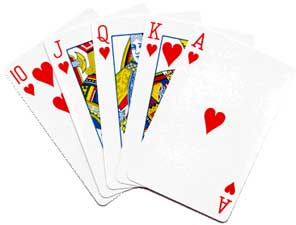
\includegraphics[width=\textwidth]{images/cartes}
%\textit{Tour de Hanoi [2]}
}%figues de la page de garde

\def\xxpied{%
Partie 5 -- Algorithmique et Programmation\\
Ch 4 : Utilisation de bibliothèques scientifiques -- \xxactivite%
}


\newcommand{\bfsf}[1]{\small\textbf{\texttt{#1}}}
\newcommand{\tsf}[1]{\small{\texttt{#1}}}
%---------------------------------------------------------------------------
\begin{document}
\chapterimage{png/Fond_ALG}
\pagestyle{empty}


%%%%%%%% PAGE DE GARDE COURS
\ifcours
\begin{tikzpicture}[remember picture,overlay]
\node at (current page.north west)
{\begin{tikzpicture}[remember picture,overlay]
\node[anchor=north west,inner sep=0pt] at (0,0) {\includegraphics[width=\paperwidth]{\thechapterimage}};
\draw[anchor=west] (-2cm,-8cm) node [line width=2pt,rounded corners=15pt,draw=ocre,fill=white,fill opacity=0.6,inner sep=40pt]{\strut\makebox[22cm]{}};
\draw[anchor=west] (1cm,-8cm) node {\huge\sffamily\bfseries\color{black} %
\begin{minipage}{1cm}
\rotatebox{90}{\LARGE\sffamily\textsc{\color{ocre}\textbf{\xxnumpartie}}}
\end{minipage} \hfill
\begin{minipage}[c]{14cm}
\begin{titrepartie}
\begin{flushright}
\renewcommand{\baselinestretch}{1.1} 
\Large\sffamily\textsc{\textbf{\xxpartie}}
\renewcommand{\baselinestretch}{1} 
\end{flushright}
\end{titrepartie}
\end{minipage} \hfill
\begin{minipage}[c]{3.5cm}
{\large\sffamily\textsc{\textbf{\color{ocre} \discipline}}}
\end{minipage} 
 };
\end{tikzpicture}};
\end{tikzpicture}


\begin{tikzpicture}[overlay]
\node[shape=rectangle, 
      rounded corners = .25 cm,
	  draw= ocre,
	  line width=2pt, 
	  fill = ocre!10,
	  minimum width  = 2.cm,
	  minimum height = 2.5cm,] at (18cm,-4.7cm) {};
\node at (17.7cm,-4.65) {\rotatebox{90}{\textbf{\Large\color{ocre}{\classe}}}};
%{};
\end{tikzpicture}

\vspace{3.5cm}

\begin{tikzpicture}[remember picture,overlay]
\draw[anchor=west] (-2cm,-6cm) node {\huge\sffamily\bfseries\color{black} %
\begin{minipage}{2cm}
\begin{center}
\LARGE\sffamily\textsc{\color{ocre}\textbf{\xxactivite}}
\end{center}
\end{minipage} \hfill
\begin{minipage}[c]{15cm}
\begin{titrechapitre}
\renewcommand{\baselinestretch}{1.1} 
\Large\sffamily\textsc{\textbf{\xxnumchapitre}}

\Large\sffamily\textsc{\textbf{\xxchapitre}}
\vspace{.5cm}

\renewcommand{\baselinestretch}{1} 
\normalsize\normalfont
\xxcompetences
\end{titrechapitre}
\end{minipage}  };
\end{tikzpicture}
\vfill

\begin{flushright}
\begin{minipage}[c]{.3\linewidth}
\begin{center}
\xxfigures
\end{center}
\end{minipage}\hfill
\begin{minipage}[c]{.6\linewidth}
\startcontents
\printcontents{}{1}{}
\end{minipage}
\end{flushright}

\begin{tikzpicture}[remember picture,overlay]
\draw[anchor=west] (4.5cm,-.7cm) node {
\begin{minipage}[c]{.2\linewidth}
\begin{flushright}

\includegraphics[width=2cm]{png/logoCC}
\end{flushright}
\end{minipage}
\begin{minipage}[c]{.2\linewidth}
\textsl{\xxauteur} \\
\textsl{\classe}
\end{minipage}
 };
\end{tikzpicture}
\newpage
\pagestyle{fancy}

\newpage
\pagestyle{fancy}

\else
\fi


%%%%%%%% PAGE DE GARDE TD
\iftd
%\begin{tikzpicture}[remember picture,overlay]
%\node at (current page.north west)
%{\begin{tikzpicture}[remember picture,overlay]
%\draw[anchor=west] (-2cm,-3.25cm) node [line width=2pt,rounded corners=15pt,draw=ocre,fill=white,fill opacity=0.6,inner sep=40pt]{\strut\makebox[22cm]{}};
%\draw[anchor=west] (1cm,-3.25cm) node {\huge\sffamily\bfseries\color{black} %
%\begin{minipage}{1cm}
%\rotatebox{90}{\LARGE\sffamily\textsc{\color{ocre}\textbf{\xxnumpartie}}}
%\end{minipage} \hfill
%\begin{minipage}[c]{13.5cm}
%\begin{titrepartie}
%\begin{flushright}
%\renewcommand{\baselinestretch}{1.1} 
%\Large\sffamily\textsc{\textbf{\xxpartie}}
%\renewcommand{\baselinestretch}{1} 
%\end{flushright}
%\end{titrepartie}
%\end{minipage} \hfill
%\begin{minipage}[c]{3.5cm}
%{\large\sffamily\textsc{\textbf{\color{ocre} \discipline}}}
%\end{minipage} 
% };
%\end{tikzpicture}};
%\end{tikzpicture}

%%%%%%%%%% PAGE DE GARDE TD %%%%%%%%%%%%%%%
%\begin{tikzpicture}[overlay]
%\node[shape=rectangle, 
%      rounded corners = .25 cm,
%	  draw= ocre,
%	  line width=2pt, 
%	  fill = ocre!10,
%	  minimum width  = 2.5cm,
%	  minimum height = 2.5cm,] at (18.5cm,0) {};
%\node at (17.7cm,0) {\rotatebox{90}{\textbf{\Large\color{ocre}{\classe}}}};
%%{};
%\end{tikzpicture}

% PARTIE ET CHAPITRE
%\begin{tikzpicture}[remember picture,overlay]
%\draw[anchor=west] (-1cm,-2.1cm) node {\large\sffamily\bfseries\color{black} %
%\begin{minipage}[c]{15cm}
%\begin{flushleft}
%\xxnumchapitre \\
%\xxchapitre
%\end{flushleft}
%\end{minipage}  };
%\end{tikzpicture}

% Bandeau titre exo
\vspace*{\espacebandeautitre}
\begin{tikzpicture}[remember picture,overlay]
\draw[anchor=west] (-2cm,-6cm) node {\huge\sffamily\bfseries\color{black} %
\begin{minipage}{5cm}
\begin{center}
\LARGE\sffamily\color{ocre}\textbf{\textsc{\xxactivite}}

\begin{center}
\xxfigures
\end{center}

\end{center}
\end{minipage} \hfill
\begin{minipage}[c]{12cm}
\begin{titrechapitre}
\renewcommand{\baselinestretch}{1.1} 
\large\sffamily\textbf{\textsc{\xxtitreexo}}

\small\sffamily{\textbf{\textit{\color{black!70}\xxsourceexo}}}
\vspace{.5cm}

\renewcommand{\baselinestretch}{1} 
\normalsize\normalfont
\xxcompetences
\end{titrechapitre}
\end{minipage}  };
\end{tikzpicture}

\else
\fi


%%%%%%%% PAGE DE GARDE FICHE
\iffiche
\begin{tikzpicture}[remember picture,overlay]
\node at (current page.north west)
{\begin{tikzpicture}[remember picture,overlay]
\draw[anchor=west] (-2cm,-3.25cm) node [line width=2pt,rounded corners=15pt,draw=ocre,fill=white,fill opacity=0.6,inner sep=40pt]{\strut\makebox[22cm]{}};
\draw[anchor=west] (1cm,-3.25cm) node {\huge\sffamily\bfseries\color{black} %
\begin{minipage}{1cm}
\rotatebox{90}{\LARGE\sffamily\textsc{\color{ocre}\textbf{\xxnumpartie}}}
\end{minipage} \hfill
\begin{minipage}[c]{14cm}
\begin{titrepartie}
\begin{flushright}
\renewcommand{\baselinestretch}{1.1} 
\large\sffamily\textsc{\textbf{\xxpartie} \\} 

\vspace{.2cm}

\normalsize\sffamily\textsc{\textbf{\xxnumchapitre -- \xxchapitre}}
\renewcommand{\baselinestretch}{1} 
\end{flushright}
\end{titrepartie}
\end{minipage} \hfill
\begin{minipage}[c]{3.5cm}
{\large\sffamily\textsc{\textbf{\color{ocre} \discipline}}}
\end{minipage} 
 };
\end{tikzpicture}};
\end{tikzpicture}


\begin{tikzpicture}[overlay]
\node[shape=rectangle, 
      rounded corners = .25 cm,
	  draw= ocre,
	  line width=2pt, 
	  fill = ocre!10,
	  minimum width  = 2.5cm,
	  minimum height = 2.5cm,] at (18.5cm,-.6cm) {};
\node at (17.8cm,-.6cm) {\rotatebox{90}{\textsf{\textbf{\large\color{ocre}{\classe}}}}};
%{};
\end{tikzpicture}



\else
\fi



%---------------------------------------------------------------------------

\def\columnseprulecolor{\color{ocre}}
\setlength{\columnseprule}{0.4pt} 

\section{Pour commencer}

\subsection{Pourquoi un cours sur \texttt{numpy}~?}

\paragraph{Le calcul scientifique} Il nécessite la manipulation de données en
quantité souvent importante. Le module \texttt{numpy} offre la
possibilité de faire du calcul de façon très efficace, reposant sur
trois principes~:

\begin{itemize}
\item 
  les données sont stockées sous la forme de tableaux \texttt{numpy},
  de type \texttt{ndarray}~;

\item 
  on utilise au maximum la manipulation de ces tableaux en évitant
  d'en faire des copies~;

\item 
  on évite si possible le recours aux boucles, préférant l'utilisation
  de fonctions \emph{vectorialisées}.
\end{itemize}

Les contraintes liées à cette volonté d'optimisations sont que les
tableaux \texttt{numpy} sont constitués d'éléments qui sont tous du
même type (en général \texttt{np.float} ou \texttt{np.int64}), et que
la taille des tableaux est fixée à la création. On ne peut donc pas
augmenter ou diminuer la taille d'un tableau~\texttt{numpy} comme on
le ferait pour une liste.

% \paragraph{L'oral de math 2 à Centrale-Supélec}
% Pour cette épreuve mixte, l'outil informatique est utilisé pour
% résoudre un exercice mathématique. C'est très naturellement que les
% bibliothèques scientifiques (\texttt{numpy},
% \texttt{matplotlib}, \texttt{scipy}) et leurs sous-modules
% (\texttt{matplotlib.pyplot}, \texttt{numpy.polynomial},
% \texttt{numpy.alg}, \texttt{scipy.integrate} etc.) sont
% utilisées. Sont annexées à ce cours les fiches fournies par le service
% concours Centrale-Supélec.

% \paragraph{L'oral de math-info aux Arts et Métiers Paristech}
% Au cours de cette épreuve, un exercice de 30~min. d'algorithmique ou
% d'ingénierie numérique est à traiter sur machine. On peut être amené
% ici aussi à utiliser des bibliothèques scientifiques. Sont annexées à
% ce cours les fiches fournies par le service concours e3a.

\subsection{Comment charger le module \texttt{numpy}~?}

On charge traditionnellement l'ensemble du module \texttt{numpy} en le
renommant éventuellement~\texttt{np}~: 

\begin{python}
import numpy as np
\end{python}

%Pour ne pas surcharger l'espace des noms et risquer la présence
%d'homonymes, on ne charge pas un module par l'instruction 
%\texttt{from module import *}.



\section{Les tableaux \texttt{numpy}}

\subsection{Création avec \texttt{np.array}}
\begin{multicols}{2}
On peut définir un tableau \texttt{numpy} à partir d'une liste, en
utilisant la fonction \texttt{array} du module~\texttt{numpy}, nommée \texttt{np.array}~: 
\begin{python}
a = np.array( [1, 2, 3] )
# [1 2 3]
b = np.array( [[1, 2, 3],
                [2, 3, 4],
                [0, 1, 0]])
# [[1 2 3]
#  [2 3 4]
#  [0 1 0]]  
\end{python}
\vspace{2cm}

Mais ce ne sont pas des listes~:
\begin{python}
print(type(a))
# <class 'numpy.ndarray'>
print(a.dtype)
# int64  
\end{python}
L'attribut \texttt{dtype} indique le type commun à tous les éléments
du tableau -- ici des entiers codés sur 64~bits.

\end{multicols}

\subsection{Création avec des fonctions spéciales}

\subsubsection{Vecteurs spéciaux (tableaux uni-dimensionnels)}

On connaît les fonctions \texttt{np.arange} et \texttt{np.linspace}~: 

\begin{multicols}{2}
\begin{python}
a = np.arange(0, 10, 2) # start, stop exclu, step
print(a)
# [0 2 4 6 8]
\end{python}
\begin{python}
b = np.linspace(0, 10, 6) # start, stop inclus, nb
print(b)
# [0. 2. 4. 6. 8. 10.]  
\end{python}
\end{multicols}
Ces fonctions sont en particulier utilisées pour le tracé des
fonctions. %Voir l'aide-mémoire annexé.



\subsubsection{Matrices spéciales (tableaux bi-dimensionnels)}

Découvrons les trois fonctions spéciales~: \texttt{np.ones},
\texttt{np.zeros}, \texttt{np.eye}, ainsi que la fonction \texttt{np.diag}~:

\begin{multicols}{2}
\begin{python}
a = np.ones((3, 5)) # Matrice de 1 3x5
# [[ 1.  1.  1.  1.  1.]
#  [ 1.  1.  1.  1.  1.]
#  [ 1.  1.  1.  1.  1.]]
b = np.ones((3, 5), np.int)
# [[1 1 1 1 1]
#  [1 1 1 1 1]
#  [1 1 1 1 1]]
c = np.zeros((3, 5)) # Matrice de 0 3x5
# [[ 0.  0.  0.  0.  0.]
#  [ 0.  0.  0.  0.  0.]
#  [ 0.  0.  0.  0.  0.]]
d = np.zeros((3, 5), dtype=np.bool)
# [[False False False False False]
#  [False False False False False]
#  [False False False False False]]
e = np.eye(3) # Matrice diagonale de 1 de taille 3x3
# [[ 1.  0.  0.]
#  [ 0.  1.  0.]
#  [ 0.  0.  1.]]  
f = np.diag([1,2,3]) # Création d'une matrice diagonale 3x3
#  définie par ... la diagonale
# [[1 0 0]
#  [0 2 0]
#  [0 0 3]]
\end{python}
\end{multicols}

\subsubsection{Tableaux aléatoires}

\begin{python}
a = np.random.randint(0, 10, size=(2, 5)) # tirage uniforme d'entiers dans [0, 10[
print(a)
# [[8 2 6 2 7]
#  [4 3 5 5 5]]
b = np.random.binomial(10, .3, (2, 5)) # simule (2, 5) valeurs d'une vad suivant une binomiale(10,.3)
print(b)
# [[1 1 2 3 3]
#  [1 2 4 2 1]]
c = np.random.geometric(.3, 5) # simule 5 valeurs d'une vad suivant une géométrique(.3)
print(c)
# [1 1 1 3 3]
d = np.random.poisson(4.3, 5) # simule 5 valeurs d'une vad suivant une poisson(4.3)
print(d)
# [2 6 6 3 3]
\end{python}

% a = np.random.rand(2, 5) # tirage uniforme dans [0,1]
% print(a)
% # [[ 0.171926    0.70301339  0.31960536  0.53837655  0.41791452]
% #  [ 0.98089744  0.57550976  0.70128171  0.61652727  0.18165619]]

% c = np.random.randn(2, 5) 
% # échantillon aléatoire au sens de la loi normale réduite (espérance 0, écart-type 1)
% print(c)
% # [[-0.08438479  0.28161157 -0.93858303  0.06438055 -0.23120253]
% #  [ 1.37703973 -0.68124     1.42005201 -0.35756701 -0.23279346]]  

% \begin{exemple}
  Comment simuler dix lancers d'un dé équilibré à~$6$ faces~?% \\
  % \texttt{np.random.randint(1,7,size=10)}
% \end{exemple}

\subsubsection{Lecture des données dans un fichier}

Si des données sont stockées dans un fichier texte avec délimiteur (format
\textsc{csv}), on peut construire la matrice de ces données avec la
fonction \texttt{np.genfromtxt}. 

\begin{multicols}{2}
Supposons que le fichier \texttt{data.csv} contienne les données suivantes~:
\begin{center}
\begin{minipage}[t]{.3\textwidth}
\lstinputlisting[frame=lbrt,frameround=ffff]{./402_numpy_data.csv}
\end{minipage}
\end{center}
On peut alors définir une matrice de la façon suivante~: 
\begin{python}
m = np.genfromtxt("./data.csv", delimiter = ',')
print (m)
# [[  1.   2.   3.   4.   5.]
#  [  6.   0.   0.   7.   8.]
#  [  0.   0.   9.  10.  11.]]  
\end{python}

\end{multicols}


\subsection{Attributs d'un tableau}
Les tableaux \texttt{numpy} sont des \texttt{objets}, qui possèdent
certains \texttt{attributs} (des propriétés de ces objets).
Modifier ces attributs est une action «~en place~», sans copie du tableau.
\begin{itemize}
\item 
  \texttt{dtype} indique le type commun de ses éléments;
\item 
  \texttt{size} indique le nombre d'éléments du tableau;
\item 
  \texttt{shape} donne le tuple de son format (nombre le lignes, de colonnes...);
\item 
  \texttt{ndim} le nombre d'indices nécessaires au parcours du tableau
  c'est-à-dire le nombre d'éléments du tuple indiquant son format.
\end{itemize}

\begin{py}
\begin{multicols}{2}
\begin{python}
a = np.array( [1, 2, 3] )
print(a.size)
# 3
print(a.shape)
# (3,)
print(a.ndim)
# 1

b = np.array( [[1, 2, 3],
               [2, 3, 4]])
print(b.size)
# 6
print(b.shape)
# (2, 3)
print(b.ndim)
# 2  
\end{python}
\end{multicols}
\end{py}

Il est remarquable que l'attribut \texttt{shape} soit mutable. On peut
aussi utiliser la méthode \texttt{reshape}.

\begin{py}
\begin{multicols}{2}
\begin{python}
b.shape = (3,2) # ou alors : b = b.reshape((3,2))
print(b)
# [[1 2]
#  [3 2]
#  [3 4]]

b.shape = (6, ) # ou alors : b.shape = (-1, )
print(b)
# [1 2 3 2 3 4]  
\end{python}
\end{multicols}
\end{py}

En fait, les éléments d'un tableau \texttt{numpy} sont stockés
consécutivement dans la mémoire, indépendamment du format. Ce n'est
que lorsque c'est nécessaire (par exemple pour l'affichage) que
l'attribut \texttt{shape} est utilisé. Modifier cet attribut est
parfaitement négligeable en terme de complexité.

L'attribut \texttt{dtype} n'est pas modifiable, puisque le stockage
d'un entier n'utilise pas le même nombre de bits que le stockage d'un
flottant ou d'un complexe. Il peut cependant être imposé à la création
du tableau \texttt{numpy}, pour éviter le casting automatique.
%
%\begin{python}
%c = np.array( [[1, 0],
%               [0, 2] ], dtype = complex)
%print(c)
%# [[ 1.+0.j  0.+0.j]
%#  [ 0.+0.j  2.+0.j]]  
%\end{python}
%
%Si l'on souhaite modifier le \texttt{dtype} d'un tableau, il faut
%passer par une copie avec conversion, en utilisant la méthode
%\texttt{astype}~: 
%\begin{python}
%d = c.astype(int)
%print(d)
%# [[1 0]
%#  [0 2]]  
%\end{python}

\subsection{Lecture dans un tableau}

\subsubsection{Slicing}
\begin{py}
\begin{multicols}{4}
  \begin{python}
a = np.array([2, 3, 5])
print(a.ndim)
# 1
print(a.shape)
# (3,)
print(a[0]) # 2
b = np.array(
 [ [2, 3, 5, 7],
 [11, 13, 17, 19],
 [23, 29, 31, 37] ])
print(b.ndim)
# 2
print(b.shape)
# (3, 4)
print(b[0,1])
# 3
print(b[:,3])
# [ 7 19 37]    
c = np.array( range(24) )
c.shape = (3, 4, 2)
print (c)
# [[[ 0  1]
#   [ 2  3]
#   [ 4  5]
#   [ 6  7]]
#  [[ 8  9]
#   [10 11]
#   [12 13]
#   [14 15]]
#  [[16 17]
#   [18 19]
#   [20 21]
#   [22 23]]]
print(c[1,:,:])
# [[ 8  9]
#  [10 11]
#  [12 13]
#  [14 15]]    
\end{python}
\end{multicols}
\end{py}

%%%%%%%%%%%%
%%%%%%%%%%%%
%\begin{center}
%\begin{tikzpicture}[scale=1]
%\foreach \x in {0,...,1}
%{   \draw (\x ,0  ,1 ) -- (\x ,3 ,1 );
%    \draw (\x ,3 ,1 ) -- (\x ,3 ,0  );
%}
%\foreach \y in {0,...,3}
%{   \draw (1 ,\y ,1 ) -- (1 ,\y ,0  );
%    \draw (0  ,\y ,1 ) -- (1 ,\y ,1 );
%}
%\foreach \z in {0,...,1}
%{   \draw (1 ,0  ,\z ) -- (1 ,3 ,\z );
%    \draw (0  ,3 ,\z ) -- (1 ,3 ,\z );
%}
%\draw[<-] (-.2,0,1) -- (-.2,3,1) node [sloped,above,midway] {\tiny \texttt{axis = 0}} ;
%% La ligne qui suit est en blanc, c'est juste pour l'alignement
%% vertical avec les figures suivantes
%\draw[->,color=white] (0,-.2,1) -- (1,-.2,1) node [sloped,below,midway] {\tiny \texttt{axis = 1}} ;
%\draw[<-] (1,2.5,.5) to [bend left] (2,3,1) node[right] {\tiny \texttt{a[0]}};
%\draw[color = black!50] (.5, 2.5, .5) node {\tiny 2};
%\draw[color = black!50] (.5, 1.5, .5) node {\tiny 3};
%\draw[color = black!50] (.5, .5, .5) node {\tiny 5};
%\end{tikzpicture}
%\begin{tikzpicture}[scale=1]
%\fill[black!20] (1,3,0) -- (1,3,1) -- (1,2,1) -- (2,2,1) -- (2,3,1) -- (2,3,0) -- cycle;
%\fill[black!10] (3,0,1) -- (4,0,1) -- (4,0,0) -- (4,3,0) -- (3,3,0) -- (3,3,1) -- cycle;
%\foreach \x in {0,...,4}
%{   \draw (\x ,0  ,1 ) -- (\x ,3 ,1 );
%    \draw (\x ,3 ,1 ) -- (\x ,3 ,0  );
%}
%\foreach \y in {0,...,3}
%{   \draw (4 ,\y ,1 ) -- (4 ,\y ,0  );
%    \draw (0  ,\y ,1 ) -- (4 ,\y ,1 );
%}
%\foreach \z in {0,...,1}
%{   \draw (4 ,0  ,\z ) -- (4 ,3 ,\z );
%    \draw (0  ,3 ,\z ) -- (4 ,3 ,\z );
%}
%\draw[<-] (-.2,0,1) -- (-.2,3,1) node [sloped,above,midway] {\tiny \texttt{axis = 0}} ;
%\draw[->] (0,-.2,1) -- (4,-.2,1) node [sloped,below,midway] {\tiny \texttt{axis = 1}} ;
%\draw[<-] (1.5,3,.5) to [bend left] (2,4,1) node[right] {\tiny \texttt{b[0,1]}};
%\draw[<-] (3.5,3,.5) to [bend left] (4,4,1) node[right] {\tiny \texttt{b[:,3]}};
%\draw[color = black!50] (.5, 2.5, .5) node {\tiny 2};
%\draw[color = black!50] (1.5, 2.5, .5) node {\tiny 3};
%\draw[color = black!50] (2.5, 2.5, .5) node {\tiny 5};
%\draw[color = black!50] (3.5, 2.5, .5) node {\tiny 7};
%\draw[color = black!50] (.5, 1.5, .5) node {\tiny 11};
%\draw[color = black!50] (1.5, 1.5, .5) node {\tiny 13};
%\draw[color = black!50] (2.5, 1.5, .5) node {\tiny 17};
%\draw[color = black!50] (3.5, 1.5, .5) node {\tiny 19};
%\draw[color = black!50] (.5, .5, .5) node {\tiny 23};
%\draw[color = black!50] (1.5, .5, .5) node {\tiny 29};
%\draw[color = black!50] (2.5, .5, .5) node {\tiny 31};
%\draw[color = black!50] (3.5, .5, .5) node {\tiny 37};
%\end{tikzpicture}
%\begin{tikzpicture}[scale=1]
%\fill[black!20] (1,3,1) -- (1,3,2) -- (1,2,2) -- (2,2,2) -- (2,3,2) -- (2,3,1) -- cycle;
%\fill[black!10] (0,1,2) -- (4,1,2) -- (4,1,0) -- (4,2,0) -- (4,2,2) -- (0,2,2) -- cycle;
%\foreach \x in {0,...,4}
%{   \draw (\x ,0  ,2 ) -- (\x ,3 ,2 );
%    \draw (\x ,3 ,2 ) -- (\x ,3 ,0  );
%}
%\foreach \y in {0,...,3}
%{   \draw (4 ,\y ,2 ) -- (4 ,\y ,0  );
%    \draw (0  ,\y ,2 ) -- (4 ,\y ,2 );
%}
%\foreach \z in {0,...,2}
%{   \draw (4 ,0  ,\z ) -- (4 ,3 ,\z );
%    \draw (0  ,3 ,\z ) -- (4 ,3 ,\z );
%}
%\draw[<-] (-.2,0,2) -- (-.2,3,2) node [sloped,above,midway] {\tiny \texttt{axis = 0}} ;
%\draw[->] (0,-.2,2) -- (4,-.2,2) node [sloped,below,midway] {\tiny \texttt{axis = 1}} ;
%\draw[->] (-.2,3.2,2) -- (-.2,3.2,0) node [sloped,above,midway] {\tiny \texttt{axis = 2}} ;
%\draw[<-] (1.5,3,1.5) to [bend left] (2,4,1) node[right] {\tiny \texttt{c[0,1,0]}};
%\draw[<-] (4,1.5,.5) to [bend right] (5,3,1) node[above] {\tiny \texttt{c[1,:,:]}};
%\draw[color = black!50] (.5, 2.5, 1.5) node {\tiny 0};
%\draw[color = black!50] (1.5, 2.5, 1.5) node {\tiny 2};
%\draw[color = black!50] (2.5, 2.5, 1.5) node {\tiny 4};
%\draw[color = black!50] (3.5, 2.5, 1.5) node {\tiny 6};
%\draw[color = black!50] (.5, 1.5, 1.5) node {\tiny 8};
%\draw[color = black!50] (1.5, 1.5, 1.5) node {\tiny 10};
%\draw[color = black!50] (2.5, 1.5, 1.5) node {\tiny 12};
%\draw[color = black!50] (3.5, 1.5, 1.5) node {\tiny 14};
%\draw[color = black!50] (.5, .5, 1.5) node {\tiny 16};
%\draw[color = black!50] (1.5, .5, 1.5) node {\tiny 18};
%\draw[color = black!50] (2.5, .5, 1.5) node {\tiny 20};
%\draw[color = black!50] (3.5, .5, 1.5) node {\tiny 22};
%\end{tikzpicture}
%\end{center}
\begin{center}
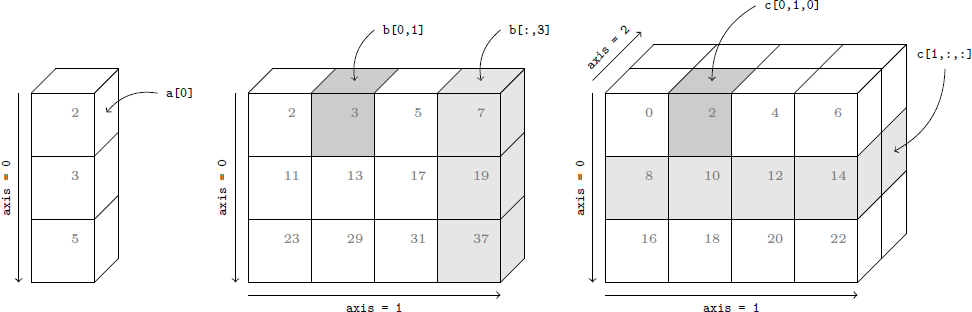
\includegraphics[width=.95\linewidth]{images/cubes}
\end{center}

\subsubsection{Les masques}

Si \texttt{a} est un tableau \texttt{numpy}, et \texttt{b} un tableau
de booléens de même format, alors \texttt{a[b]} met en relation un à
un les éléments de \texttt{a} et ceux de \texttt{b}, en ne conservant
que les éléments de~\texttt{a} associés à la valeur \texttt{True}~:
\begin{python}
a = np.array(range(10))
a.shape = (2, 5)
print(a)
b = np.array([[ True, False, False,  True, False],
              [False,  True, False, False,  True]])
print(a[b])
# [0 3 6 9]  
\end{python}

On verra au §~\ref{operations} qu'il est aisé de construire le tableau
des booléens traduisant par exemple la propriété~: l'élément est
divisible par~$3$.

\begin{python}
b = a % 3 == 0
print(b)
[[ True False False  True False]
 [False  True False False  True]]  
\end{python}

Bref, pour obtenir tous les éléments de~\texttt{a} qui sont divisibles
par~$3$, on écrira donc~: 
\begin{python}
a [ a % 3 == 0 ]  
\end{python}

\subsection{Écriture dans un tableau}

Les tableaux \texttt{numpy} sont mutables, on peut donc modifier les
valeurs qu'ils contiennent sans redéfinir l'objet lui-même. Et on peut
modifier simultanément plusieurs valeurs, en utilisant les mêmes
syntaxes qu'au paragraphe précédent.

\begin{py}
\begin{multicols}{4}
\begin{python}
a = np.array(range(10))
a.shape = (2, 5)
print(a)
# [[0 1 2 3 4]
#  [5 6 7 8 9]]
a[0,0] = 7
print(a)
# [[7 1 2 3 4]
#  [5 6 7 8 9]]
a[0,:] = [8, 7, 6, 5, 4]
print(a)
# [[8 7 6 5 4]
#  [5 6 7 8 9]]
a[ a % 2 == 0 ] /= 2
print(a)
# [[4 7 3 5 2]
#  [5 3 7 4 9]]  
\end{python}
\end{multicols}
\end{py}
Dans ce dernier exemple, les éléments pairs de~\texttt{a} sont divisés
par~$2$.
% Importance du /= et non / :
%avec / : renvoie array([ 4.,  3.,  2.,  3.,  4.])
%puis avec le print(a) : a pas modifié ([[8 7 6 5 4][5 6 7 8 9]])

\subsection{À propos des copies}
Lorsque l'on manipule de grandes quantités de données, c'est souvent
une mauvaise idée de vouloir copier ces données. C'est pourquoi la
plupart des manipulations de tableau \texttt{numpy} se fait au travers
de~\emph{vues} d'un même tableau.

\begin{python}
a = np.array(range(10))
a.shape = (2, 5)
b = a
print(id(a), id(b))
# 4346543408 4346543408  
\end{python}
Ici, comme on pouvait s'y attendre, \texttt{a} et \texttt{b} sont
simplement deux noms pour un même objet.


% Lorsque l'on manipule des
%listes, on peut faire~: 
%\begin{python}
%b = a[:,:]
%print(id(a), id(b))
%# 4346543408 4299979904  
%\end{python}
%ce qui apparaît comme prometteur~: \texttt{a} et \texttt{b} ne
%correspondent plus à un même objet. Cependant~:
%\begin{python}
%b.fill(1)
%print(a)
%# [[1 1 1 1 1]
%#  [1 1 1 1 1]]
%print(b)
%# [[1 1 1 1 1]
%#  [1 1 1 1 1]]  
%\end{python}
%
%De même~: 
%\begin{python}
%a = np.zeros((2, 5), dtype=np.int64)
%b = a[1, 1:3]
%b[:] = [1, 1]
%print(a)
%# [[0 0 0 0 0]
%#  [0 1 1 0 0]]  
%\end{python}
%
%\texttt{a} et \texttt{b} sont en fait deux \emph{vues} (partielle
%pour~\texttt{b}) du même objet. 

\begin{remark}
C'est en général une mauvaise idée, mais si on souhaite malgré tout
faire une copie d'un tableau \texttt{numpy}, on utilise la méthode
\texttt{copy()}, ou bien \texttt{astype(\textit{dtype})} déjà
mentionnée.
\end{remark}

\section{Opérations sur les tableaux \texttt{numpy}}

\subsection{Les opérations se font terme à terme}
\label{operations}
Les opérations \texttt{+}, \texttt{*}, \texttt{/}, \texttt{==}, etc s'appliquent aux tableaux
\texttt{numpy}, mais \emph{TERME à TERME}. C'est cohérent avec la
définition mathématique pour l'addition, mais ça ne l'est plus du tout
pour la multiplication, les puissances etc.
\begin{py}
\begin{multicols}{2}
\begin{python}
a = np.random.randint(0, 10, (2, 5))
b = np.random.randint(1, 10, (2, 5))
print(a)
# [[0 9 0 6 6]
#  [8 9 2 0 0]]
print(b)
# [[3 1 3 5 2]
#  [8 7 7 1 6]]
print(a + b)
# [[ 3 10  3 11  8]
#  [16 16  9  1  6]]
print(a * b)
# [[ 0  9  0 30 12]
#  [64 63 14  0  0]]
print(a // b)
# [[0 9 0 1 3]
#  [1 1 0 0 0]]
print(a / b)
# [[ 0.          9.          0.          1.2         3.        ]
#  [ 1.          1.28571429  0.28571429  0.          0.        ]]
print(a ** b)
# [[       0        9        0     7776       36]
#  [16777216  4782969      128        0        0]]  
print(a == b)
# [[False False False False False]
#  [True False False False False]]
\end{python}
\end{multicols}
\end{py}

\subsection{Les fonctions universelles s'appliquent terme à terme}
Les fonctions définies dans le module \texttt{numpy} sont
\emph{universelles}, ou \emph{vectorialisées}, c'est-à-dire qu'elles acceptent comme argument un
tableau \texttt{numpy} et renvoient le tableau \texttt{numpy} des
images. Utiliser des fonctions vectorialisées permet de faire gagner
des facteurs énormes en temps de calcul.

\begin{python}
x = np.linspace(-1, 1, 18)
y = np.arcsin(x)
print(y)
# [-1.57079633 -1.080839   -0.87058477 -0.70372051 -0.55790704 -0.42438971
#  -0.2985322  -0.1773996  -0.05885751  0.05885751  0.1773996   0.2985322
#   0.42438971  0.55790704  0.70372051  0.87058477  1.080839    1.57079633]  
\end{python}

On peut vectoriser ses propres fonctions~:
\begin{python}
def f(x):
    k, s = 0, 0
    while s <= x:
        k += 1
        s += k
    return k

print(f(9.56))
# 4

x = np.arange(1, 10, 2)
# print(f(x)) # déclenche une erreur
vf = np.vectorize(f)
print(vf(x))
# [2 3 3 4 4]  
\end{python}

\subsection{Quelques méthodes sur les tableaux}
On peut utiliser les méthodes (ou les fonctions associées)
\texttt{a.max()}, 
\texttt{a.min()}, 
\texttt{a.sum()}, 
\texttt{a.prod()}, 
\texttt{a.mean()} (moyenne arithmétique), 
\texttt{a.var()} (variance), 
\texttt{a.std()} (écart-type).

\begin{py}
\begin{multicols}{3}
\begin{python}
a = np.random.randint(0, 10, (2,5))
print(a)
# [[8 5 0 1 3]
#  [2 2 1 5 3]]
print(a.sum()) #ou encore np.sum(a)
# 30
print(a.sum(axis=0))
# [10  7  1  6  6]
print(a.sum(axis=1))
# [17 13]
print(a.mean())
# 3.0
print(a.mean(axis=0))
# [ 5.   3.5  0.5  3.   3. ]
print(a.mean(axis=1))
# [ 3.4  2.6]
print(a.max())
# 8
print(a.max(axis=0))
# [8 5 1 5 3]
print(a.max(axis=1))
# [8 5]  
\end{python}
\end{multicols}
\end{py}

\subsection{Opérations d'algèbre linéaire}

Commençons par le produit matriciel~: c'est la fonction
\texttt{np.dot(a,b)} ou la méthode \texttt{a.dot(b)}~:

\begin{py}
\begin{multicols}{3}
\begin{python}
a = np.array([[1,2,3],
              [4,5,6],
              [7,8,9]])
b = np.array([[0,1,0],
              [1,0,0],
              [0,0,1]])
print(np.dot(a,b)) 
# ou alors print(a.dot(b))  
# [[2 1 3]
#  [5 4 6]
#  [8 7 9]]
\end{python}
\end{multicols}
\end{py}


\begin{itemize}
\item Le produit scalaire canonique, entre deux vecteurs ou deux matrices,
se calcule avec \texttt{np.vdot}.
\item Le produit vectoriel se calcule avec \texttt{np.cross}.
\item La transposée de la matrice \texttt{a} est \texttt{a.transpose()} ou
plus simplement \texttt{a.T}.
\item Le sous-module \texttt{linalg} fournit les fonctions~:
%\begin{center}
  \texttt{np.linalg.det}, \texttt{np.linalg.inv},
  \texttt{np.linalg.norm}, \texttt{np.linalg.solve},\\
  \texttt{np.linalg.matrix\_power},
  \texttt{np.linalg.matrix\_rank};
dont les
significations sont immédiates. Pour cette dernière, la matrice doit
être inversible pour que le résultat soit cohérent.
\end{itemize}
\begin{multicols}{2}
\begin{python}
a = np.array([[1,2,3],
              [0,2,2],
              [0,2,3]])
b = np.array([4,9,1])
print(np.linalg.solve(a,b))
# [  3.   12.5  -8. ]  
\end{python}
\end{multicols}
 
La fonction \texttt{np.linalg.eig} fournit un couple de deux matrices,
la première étant le spectre de la matrice, donné sous forme d'un
vecteur où les valeurs propres multiples apparaissent autant de fois
que leurs multiplicités, et d'une matrice carrée dont les colonnes
sont des vecteurs engendrant respectivement les espaces propres de la
matrice. On utilisera cette fonction dans le chapitre de mathématique
concernant la réduction des matrices.

\begin{multicols}{2}
\begin{python}
a = np.array([[1,2,3],
              [0,1,2],
              [0,0,2]])
sp, p = np.linalg.eig(a)
print(sp)
# [ 1.  1.  2.]
print(p)
# [[ 1.00000000e+00 -1.00000000e+00   9.52579344e-01]
#  [ 0.00000000e+00   1.11022302e-16   2.72165527e-01]
#  [ 0.00000000e+00   0.00000000e+00   1.36082763e-01]]  
\end{python}
\end{multicols}
%
%Terminons par des opérations sur les tableaux~:
%\texttt{np.concatenate((a,b), axis=0)} permet d'accoler les tableaux
%\texttt{a} et \texttt{b} dans la direction
%indiquée. \texttt{np.column\_stack((v1,v2,v3))} permet de construire
%la matrice dont les colonnes sont les vecteurs passés en arguments.
%
%\begin{multicols}{3}
%\begin{python}
%a = np.array([[1,2,3],
%              [4,5,6],
%              [7,8,9]])
%b = np.array([[0,1,0],
%              [1,0,0],
%              [0,0,1]])
%print(np.concatenate((a,b),axis=0))
%# [[1 2 3]
%#  [4 5 6]
%#  [7 8 9]
%#  [0 1 0]
%#  [1 0 0]
%#  [0 0 1]]
%print(np.concatenate((a,b),axis=1))
%# [[1 2 3 0 1 0]
%#  [4 5 6 1 0 0]
%#  [7 8 9 0 0 1]]
%
%v1 = np.array([1,2,3])
%v2 = np.array([4,5,6])
%v3 = np.array([1,0,0])
%p = np.column_stack((v1,v2,v3))
%print(p)
%# [[1 4 1]
%#  [2 5 0]
%#  [3 6 0]]  
%\end{python}
%\end{multicols}

\subsection{Manipulation de polynômes}

Une classe \texttt{Polynomial} est disponible, et permet de manipuler
les polynômes, qui sont représentés à l'aide de la liste des
coefficients classés par ordre croissant de degré. L'objet créé a un
attribut \texttt{coef}, des méthodes \texttt{degree}, \texttt{roots},
\texttt{deriv}, \texttt{integ} permettant d'accéder respectivement au degré, à des
valeurs approchées de racines, à la dérivée formelle, à une primitive
formelle. On peut aussi utiliser l'objet pour évaluer la fonction
polynomiale associée.

\begin{multicols}{2}
\begin{python}
from numpy.polynomial import Polynomial

p = Polynomial([1, 0, 1])
# ou alors, plus commode pour travailler formellement : 
X = Polynomial([1, 0])
p = X ** 2 + 1 
print(p.coef)
# [ 1.  0.  1.]
print(p.degree())
# 2
print(p.roots())
# [ 0.-1.j  0.+1.j]
dp = p.deriv()
print(dp.coef)
# [ 0.  2.]
ip = p.integ()
print(ip.coef)
# [ 0.          1.          0.          0.33333333]  
print(p(0))
# 1.0
print(p(0+1j))
# 0j
\end{python}
\end{multicols}
\begin{thebibliography}{2}
\bibitem{1}{Guillaume Haberer, \textit{Supports de cours de PSI $\star$}, Lycée La Martinière Monplaisir, Lyon.}

\end{thebibliography}
\end{document}

